\paragraph{1. Dependancy toevoegen}
Normaal zijn bevatten alle projecten gestart met Android Studio de nodige dependancies om de NotificationCompat API
te gebruiken. Maar voor de zekerheid verifiëren we dat onderstaande dependancy er bij zit.
\begin{minted}{java}
  val core_version = "1.6.0"
  dependencies {
      implementation("androidx.core:core-ktx:$core_version")
  }
\end{minted}
Als de dependancy is toegevoegd dan kunnen we notificaties beginnen aanmaken.

\paragraph{2. Notificatie aanmaken}
Om een notificatie aan te maken gaan we het NotificationCompat.Builder object gebruiken. 
\begin{minted}{kotlin}
  private fun createNotification(title: String, body: String) {
    val builder = NotificationCompat.Builder(this, CHANNEL_ID)
      .setSmallIcon(icon)
      .setContentTitle(title)
      .setContentText(body)
      .setPriority(NotificationCompat.PRIORITY_DEFAULT)

    val notificationManager: NotificationManager =
      getSystemService(Context.NOTIFICATION_SERVICE) as NotificationManager
    notificationManager.notify(notificationId, builder.build())
}
\end{minted}
\begin{figure}[H]
    \centering
    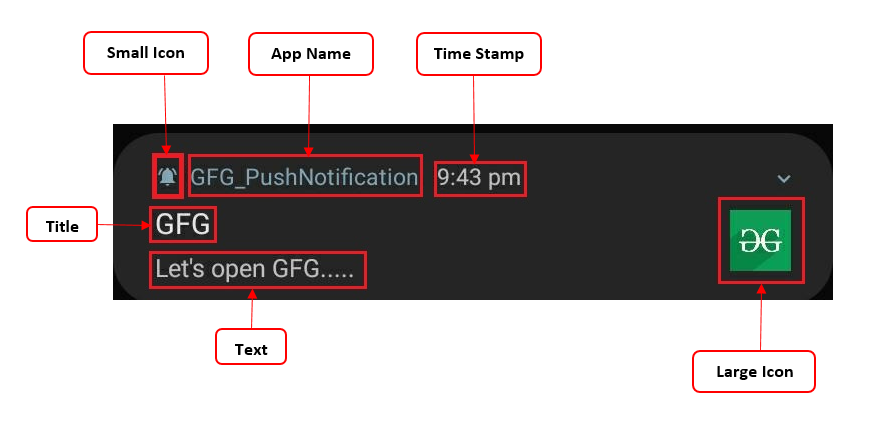
\includegraphics[height=0.3\textheight]{NotificationAnatomy.png}
    \caption{Anatomy standaard notificatie \parencite{One2020}.}
\end{figure}

\paragraph{3. Channel aanmaken}
Het laatste dat we nodig hebben vooraleer de notificatie getoond kan worden is een channel. Deze worden 
gebruikt om notificaties te groeperen volgens hun belang. Om een channel aan te maken gebruiken we 
de .createNotificationChannel() methode. Het maakt niet uit wanneer of waar deze code wordt uitgevoerd. 
Het is enkel belangrijk dat de channel wordt aangemaakt vooraleer er wordt geprobeerd om notificaties 
te tonen. Dus best zo vroeg mogelijk in de applicatie.
\begin{minted}{kotlin}
private fun createNotificationChannel() {
  if (Build.VERSION.SDK_INT >= Build.VERSION_CODES.O) {
    val name = "bachproef"
    val descriptionText = "bachproef notificaties"
    val importance = NotificationManager.IMPORTANCE_DEFAULT
    val channel = NotificationChannel(CHANNEL_ID, name, importance).apply {
      description = descriptionText
    }
    // Channel bij het systeem registreren
    val notificationManager: NotificationManager =
      getSystemService(Context.NOTIFICATION_SERVICE) as NotificationManager
    notificationManager.createNotificationChannel(channel)
  }
}
\end{minted}

\paragraph{4. Applicatie maken}
Met deze informatie kunnen we nu een applicatie opbouwen die notificaties zal sturen. De applicatie bestaat 
uit twee \textbf{EditText} componenten voor een titel en beschijving van de notificatie en tot slot een 
\textbf{Button} om de notificatie te triggeren. Als de knop wordt ingedrukt dan wordt de 
\textbf{createNotification} methode aangeroepen en wordt de waarde van de inputs meegegeven.
\begin{figure}[H]
  \centering
  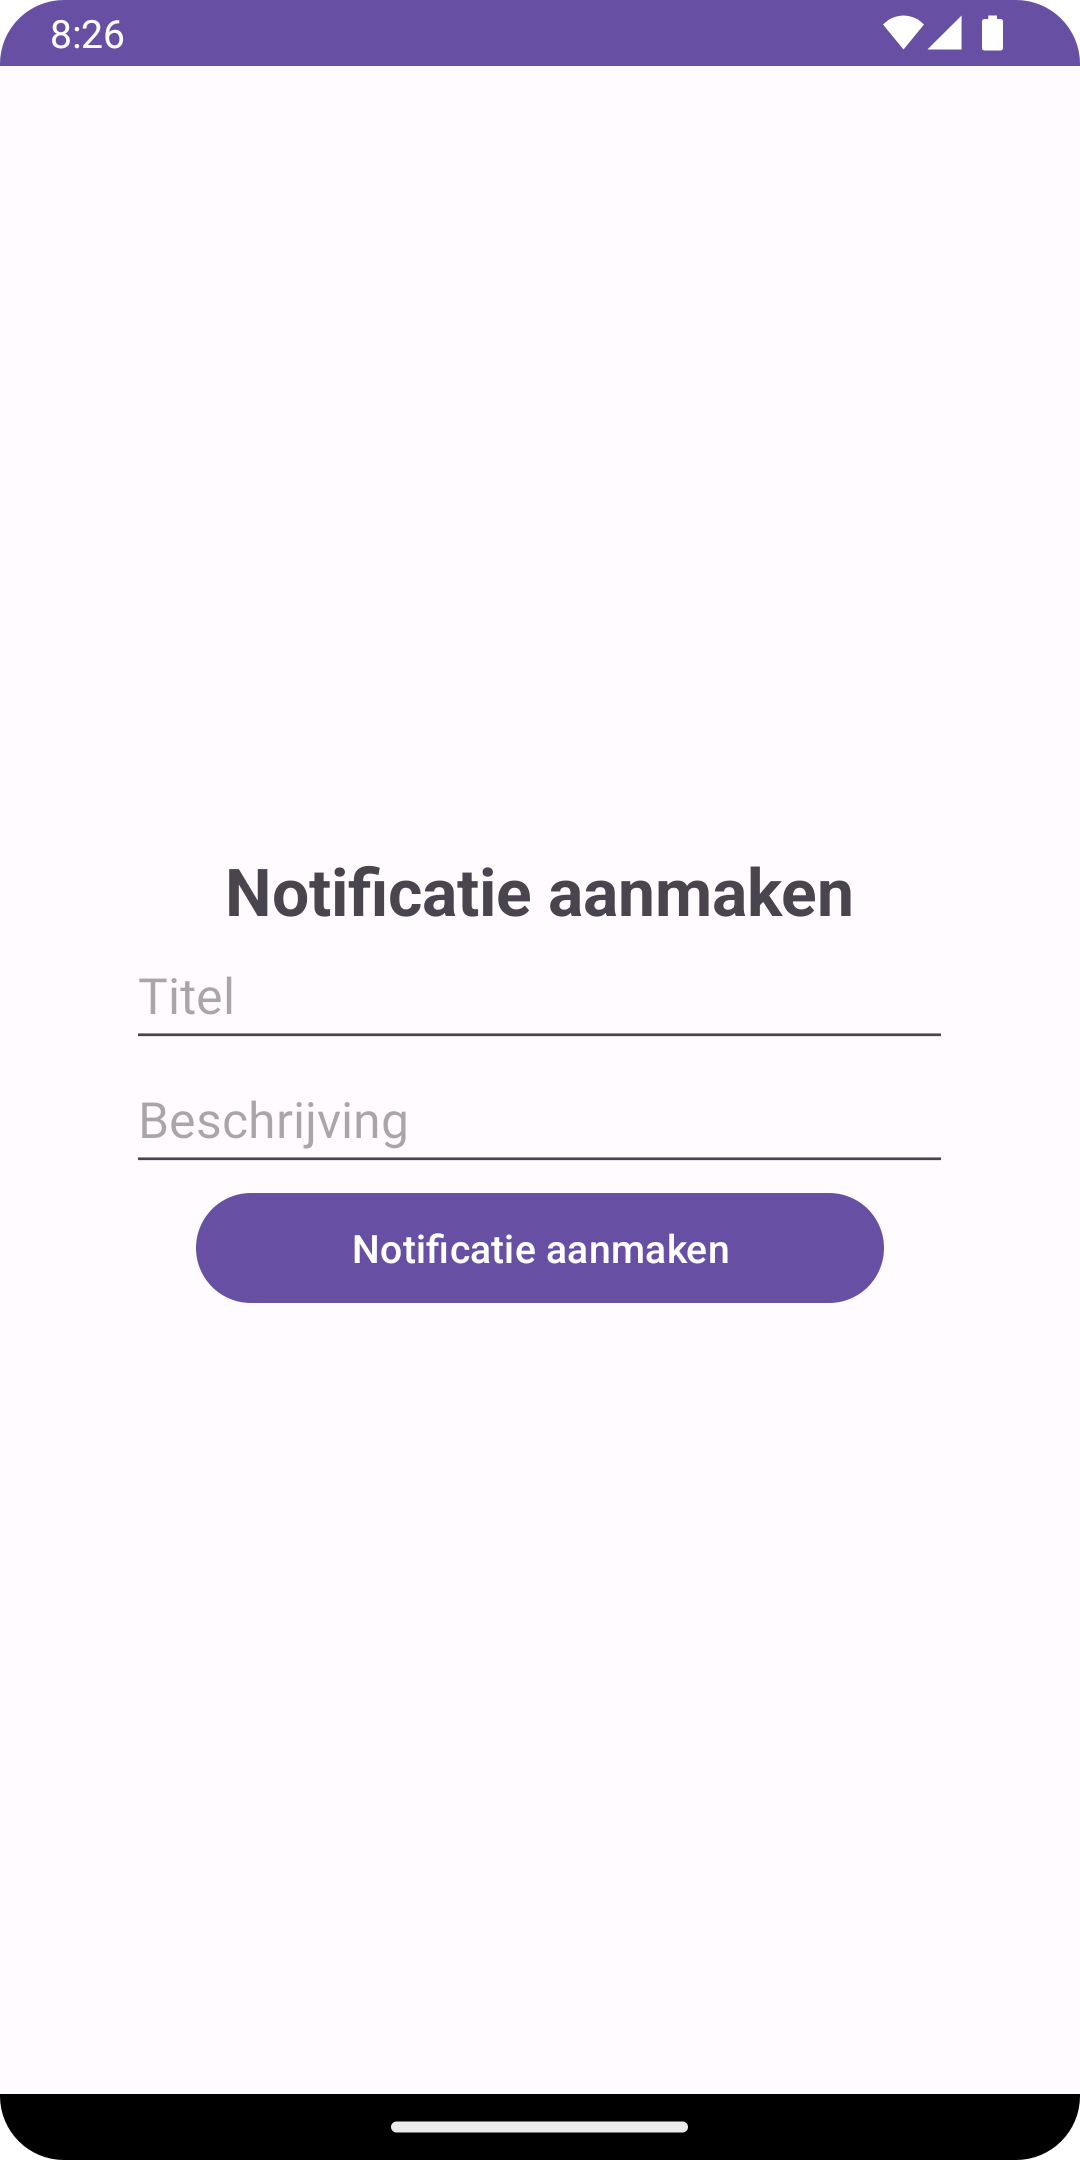
\includegraphics[height=0.5\textheight]{notificaties_layoutnative.png}
  \caption{Layout van applicatie voor notificaties te sturen bij Android.}
\end{figure}